38. \begin{figure}[ht!]
\center{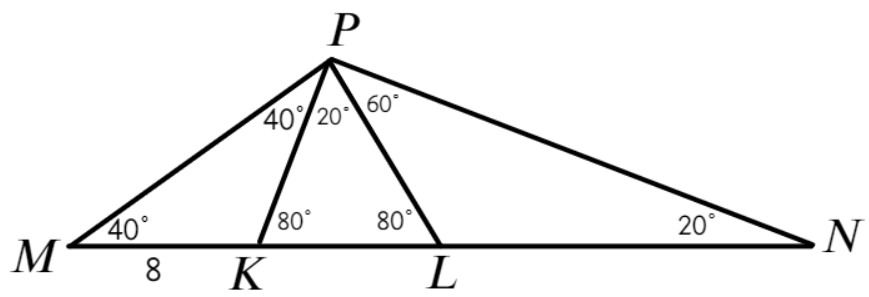
\includegraphics[scale=0.35]{g38.png}}
\end{figure}\\
Пусть $PL$ --- биссектриса. Сделаем дополнительное построение: отметим на стороне $MN$ точку $K$ так, чтобы $NP=NK.$ Тогда $MK=MN-NK=MN-NP=8.$ Треугольник $PNK$ является равнобедренным с углом при вершине $20^\circ,$ значит $\angle PKN=\angle KPN=(180^\circ-20^\circ):2=80^\circ.$ Угол $P$ равен $180^\circ-20^\circ-40^\circ=120^\circ,$ значит $\angle LPN=120^\circ:2=60^\circ,\ \angle KPL=80^\circ-60^\circ=20^\circ,\ \angle MPK=60^\circ-20^\circ=40^\circ,\ \angle PLK=180^\circ-20^\circ-80^\circ=80^\circ.$ Таким образом, треугольники $MPK$ и $KPL$ являются равнобедренными, а поэтому $PL=PK=MK=8.$\newpage
\noindent39. \begin{figure}[ht!]
\center{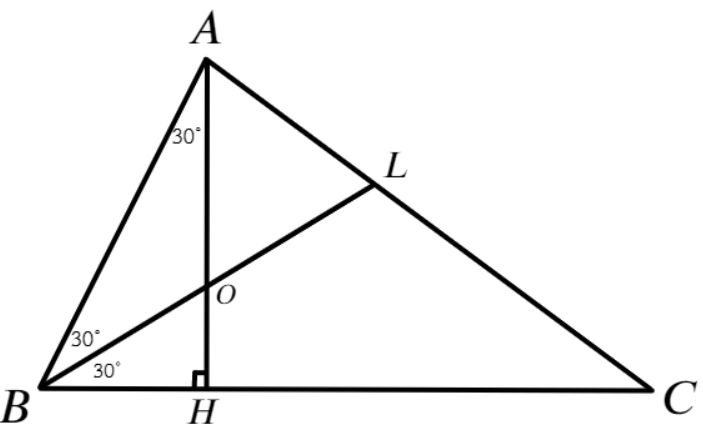
\includegraphics[scale=0.35]{g39.png}}
\end{figure}\\
Пусть $BL$ и $AH$ пересекаются в точке $O.$ Так как $BL$ является биссектрисой, $\angle OBH=\angle OBA=30^\circ.$ Из треугольника $ABH:\ \angle BAH=180^\circ-90^\circ-60^\circ=30^\circ.$ В прямоугольном треугольнике $OBH$ катет $BH$ лежит напротив угла в $30^\circ,$ поэтому $OB=2OH.$ В треугольнике $OBA$ равны углы при стороне $AB,$ значит он является равнобедренным и $AO=OB.$ Таким образом, $AO:OH=OB:OH=2OH:OH=2:1.$\\
